\documentclass{article}
\usepackage[utf8]{inputenc}
\usepackage{listings}
\usepackage{graphicx}
\usepackage{float}
\usepackage{xcolor}
\usepackage{geometry}
\usepackage{CJKutf8}
\usepackage{amsmath}
\usepackage{amssymb}

\geometry{a4paper,scale=0.8}
\lstset{
    basicstyle          =   \sffamily,        
    keywordstyle        =   \bfseries,         
    commentstyle        =   \rmfamily\itshape, 
    stringstyle         =   \ttfamily, 
    flexiblecolumns,               
    numbers             =   left,  
    showspaces          =   false, 
    showstringspaces    =   false,
    captionpos          =   t,     
    frame               =   lrtb, 
}

\lstdefinestyle{Python}{
    language        =   Python, % 语言选Python
    basicstyle      =   \zihao{-5}\ttfamily,
    numberstyle     =   \zihao{-5}\ttfamily,
    keywordstyle    =   \color{blue},
    keywordstyle    =   [2] \color{teal},
    stringstyle     =   \color{magenta},
    commentstyle    =   \color{red}\ttfamily,
    breaklines      =   true,  
    columns         =   fixed,  
    basewidth       =   0.5em,
}

\title{\bf\Large  分支过程:从一道作业题出发}
%%%%%%%%%%%%%%%%%%%%%%%%%%%%%%%%%%%%%%
%% DON'T forget to change this part %%
\author{\bf Name: 宋昊原 \qquad Student ID: 2022010755}
%%%%%%%%%%%%%%%%%%%%%%%%%%%%%%%%%%%%%%

\begin{document}
\begin{CJK}{UTF8}{gbsn}
\maketitle
\textbf{习题2-11}\ \ \  有一个生物,1分钟后有三种可能结果:死掉、保持原状或者分裂成两个,出现的概率都相同,而此后活着的该种生物都将以这种方式相互独立地进行下去,那么这种生物最终灭亡的概率是多少?
\section{简单的分析}
当时我在作业中的分析是这样的:设该生物最终灭亡的概率为$p$,则根据各代之间独立性,有
$$ p = \frac{1}{3}+\frac{1}{3}p+\frac{1}{3}p^{2} $$
解得
$$ p=1 $$
即该生物注定灭亡.
\section{追加的补充逻辑}
然而,上面的分析过于简单,这里还需要增加一下对设出$p$并应用该等式的合理性的讨论:
\\\\
设该生物经过$n$代后灭亡的概率是$p_{n}$,由于此时并不涉及“最终灭亡”这样可能永远不会产生结果的极限命题,这个定义是合理的.\ \ 此时根据全概率公式有
$$ p_{n} = \frac{1}{3}+\frac{1}{3}p_{n-1}+\frac{1}{3}p_{n-1}^{2},\ \forall n\geq 1 $$
$$ p_{0} = 0 $$
则
$$ p_{n}-p_{n-1}=\frac{1}{3}(1-p_{n-1})^{2}\geq 0 $$
即数列$\{p_{n}\}_{n=0}^{\infty}$单调递增且有上界$1$,于是收敛,设其极限为$p$,对上述递推式取极限得到最初讨论中的式子
$$ p = \frac{1}{3}+\frac{1}{3}p+\frac{1}{3}p^{2} $$
这保证了上面分析在逻辑上的成立.
\section{潜在的问题}
上面的讨论可以解决这个问题,然而,注意到上面的方程
$$ p = \frac{1}{3}+\frac{1}{3}p+\frac{1}{3}p^{2} $$
有二重根$p=1$,而如果改变方程的一些系数(即不同情况发生的概率),方程不一定总是有二重根,如果其在$[0,1]$范围内有多个不同的根应当取哪一个?
\\\\
回顾之前的讨论会发现,这里只是给出了极限概率$p$应满足的必要条件,并没有给出其充分条件,所以同时解出多个合理解是可能的.
\\\\
例如,如果该生物不会死掉,而是保持一个、变成两个的概率各一半,则上述方程变为
$$ p=\frac{1}{2}p+\frac{1}{2}p^{2} $$
解得$p=0$或$p=1$.\ \ 显然这里生物不存在灭绝的可能,应当取$p=0$作为合理解,但这是为什么?事实上,习题课中给出的结论是,如果此方程存在多个解,应当取较小的.\ \ 下面我将根据参考文献中提到的书目《概率论及其应用》来进一步分析这个问题.
\section{分支过程与概率母函数}
我们讨论的分支过程是以下的情景:
\\\\
\textbf{定义(分支过程)}每一个体经过一个时间周期后有$p_{k}$的概率变成$k$个($k\in\mathbb{N},\ \sum\limits_{k=1}^{\infty}p_{k}=1$),不同个体的变化是独立的,考虑一个初始个体经过若干周期后的结果.
\\\\
\textbf{定义(概率母函数)}对离散随机变量$X$,设其全部可能取值为$n=0,1,2,...$,对应概率为$\{p_{n}\}_{n=0}^{\infty}$,则其概率母函数定义为
$$P(s)=\sum\limits_{n=0}^{\infty}p_{n}s^{n}$$
\\\\
此定义实际上很类似于课上有过详细讨论的矩母函数,事实上这种情况下的矩母函数为
$$ M_{X}(t)=\sum\limits_{n=0}^{\infty}p_{n}{\rm e}^{nt}=P({\rm e}^{t}) $$
接下来考虑概率母函数与分支过程的关系.
\\\\
设$Z_{n}$为经过$n\in\mathbb{N}$个周期后剩余的个体数,并且设$Z_{n}$的概率母函数为$P_{n}(s)$,上述分支过程一个个体的后代分布的概率母函数为$P(s)$,则有
$$ P_{0}(s) = s $$
$$ P_{n}(s) = P(P_{n-1}(s)),\ n\in\mathbb{N}_{+} $$
其中$P_{0}$的结果是由$Z_{0}\equiv 1$得到的,下面我将证明上述递推公式.
\section{递推公式的证明}
首先,与矩母函数$M_{X}(t)={\rm E}({\rm e}^{Xt})$类似,概率母函数$P_{X}(s)={\rm E}(s^{X})$.\ \ 故,如果$X$与$Y$独立,其概率母函数也满足:
$$ P_{X+Y}(s)={\rm E}(s^{X+Y})={\rm E}(s^X){\rm E}(s^Y)=P_X(s)P_Y(s) $$
同时,设${\{B_{k}\}}_{k=0}^{\infty}$是对样本空间的一个划分,${\rm P}(B_k)=p_k$,则根据全概率公式有
$$ {\rm P}(X=m)=\sum\limits_{k=0}^{\infty}p_k{\rm P}(X=m|B_k) $$
于是,如果设$X$的概率母函数为$P(s)$,在$B_k$发生的情况下$X$的条件概率母函数为$P_{B_k}(s)$,则对$P(s)$每一项,上述全概率公式成立,于是整体地有
$$ P(s)=\sum\limits_{k=0}^{\infty}p_k P_{B_k}(s) $$
即概率母函数也满足类似的全概率公式.
\\\\
至此,对于上面定义的$Z_n$的概率母函数$P_n(s)$,可以按照第一代产生的个体数$k$讨论,由于独立随机变量之和的概率母函数是对应概率母函数是乘积,这$k$个个体经$n-1$代产生的个体数的概率母函数为
$$ (P_{n-1}(s))^k $$
根据概率母函数的全概率公式有
$$ P_n(s)=\sum\limits_{k=0}^{\infty}p_{k}(P_{n-1}(s))^k=P(P_{n-1}(s)) $$
\section{灭绝概率}
接下来讨论题目中的灭绝概率,设经过$k$代后灭绝的概率是$x_k$,则$x_k$为$P_k(s)$的常数项,即
$$ x_k=P_k(0)=P(P_{k-1}(0))=P(x_{k-1}) $$
同时满足$x_0=0$,$x_1=p_0$.
\\\\
上面已经讨论过,$\{x_k\}$单调递增且有上界,于是有极限$x$,且$x$满足$x=P(x)$.
\\\\
在区间$[0,1]$上,函数$P(s)$始于$(0,p_0)$,终于$(1,1)$,且由于其系数均正,$P(s)$是下凸的增函数,除去个别平凡情形(如$P(s)\equiv s$)外,$P(s)$曲线在$[0,1]$上与坐标系主角平分线至多两个交点,且其中一个是$(1,1)$.
\\\\
\textbf{情形 1}\ \ \ 若$(1,1)$是唯一的交点,则$x=1$,注定灭绝,此时$P(s)$曲线如下图所示:\\\\
\begin{minipage}{0.5\textwidth}
    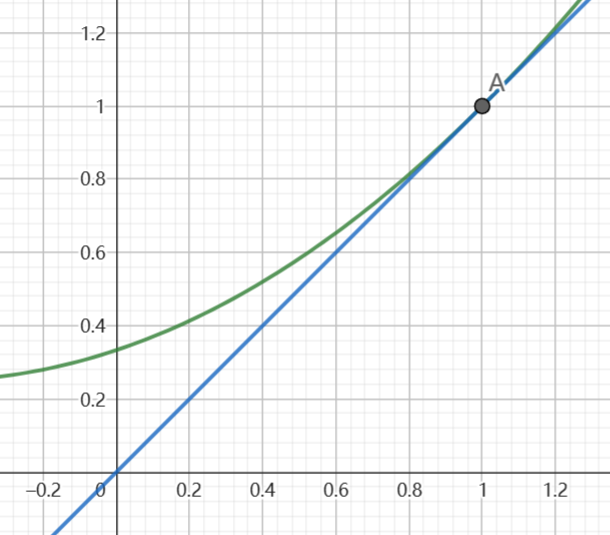
\includegraphics[scale=0.7]{case1.png}
\end{minipage}
\\\\
\textbf{情形 2}\ \ \ 若除了$(1,1)$外还有一个交点$(s_0,s_0)$,则根据$P(s)$单调性和$P(s_0)=s_0$,有
$$ x_1=p_0=P(0)<P(s_0)=s_0 $$
$$ x_2=P(x_1)<P(s_0)=s_0 $$
类推可知,$x_k$总在$s_0$左侧,于是
$$ x=s_0 $$
这证明了灭绝概率总是取可能解中较小者,图示如下:\\\\
\begin{minipage}{0.5\textwidth}
    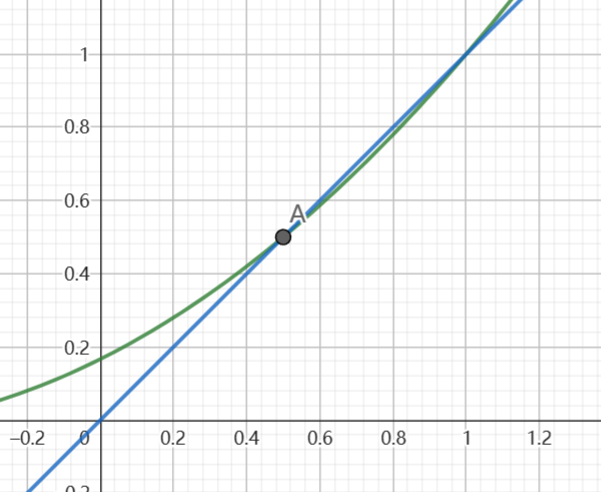
\includegraphics[scale=0.7]{case2.png}
\end{minipage}
\section{灭绝概率与期望后代数}
注意到
$$ P'(1)=\sum\limits_{k=0}^{\infty}kp_{k}={\rm E}(Z_1)=\mu $$
即$P'(1)$是一个个体的期望后代数$\mu$.
\\\\
回顾上一部分中给出的两幅示意图,根据函数下凸这一性质容易发现,$\mu\leq 1$时出现情况1,而$\mu>1$时出现情况2(除去$p_1=1$,即此生物永不改变的这一平凡情况以外).
\\\\
于是,除去上述平凡情况,可以根据每个个体平均后代数$\mu$的大小来判断灭绝概率,若$\mu<1$则必定灭绝,因为该种群数量期望地减少,$\mu>1$则有一定概率不灭绝(但仍有一定概率$x$是会灭绝的,除非$p_0=0$).\ \ 较反直觉的是,$\mu=1$时同样必定灭绝.\ \ 这可以理解为,尽管种群数量期望上不变,但灭绝概率却是严格单增的,于是这会导致随着代数增加,越来越大的概率灭绝,而较小概率未灭绝的种群则可能有超大的种群数量.
\\\\
上面的讨论实际上忽略了一点,就是$\mu$作为一个期望本身可以是无穷的.\ \ 这样的例子很容易构造,例如,一个个体有$1/2$概率死亡,$1/4$概率不变,$1/8$概率变成两个,$1/16$概率变成四个,类似地,$1/2^{n+2}$概率变成$2^n$个.\ \ 则此时
$$ \mu=\frac{1}{4}+\frac{1}{4}+\frac{1}{4}+...=+\infty $$
然而此生物仍然可能灭绝,经过计算器计算,在最大的一项取到$x^{256}/1024$的情况下,灭绝概率$x$以至少$10^{-10}$的精度收敛于$0.8336$,这仍是一个很高的概率,这再度佐证了极端值存在的情况下期望作为唯一的判据并不是那么可信.
\section{实验:期望灭绝时间}
这里定义$T$为种群数量第一次归零的轮次,设$P(T=k)=t_k$,则
$$ t_1 = x_1 $$
$$ t_k = x_k-x_{k-1} $$
于是
$$ {\rm E}(T)=\sum\limits_{k=1}^{\infty}kt_k=\lim_{n\to\infty}(nx_n-(x_1+...+x_{n-1})) $$
进而可以用下面的Python代码来估算在不同的概率母函数$p(x)$的情况下的${\rm E}(T)$的值,可以通过调整$n$的值观察估计值的变化来判断此期望是否收敛.
\begin{center}
    \lstset{language=Python}
    \begin{lstlisting}
def p(x):
    return 1/3 + x/3 + x**2/3
n = 100000
prob = []
prob.append(p(0))
for i in range(n):
    prob.append(p(prob[i]))
sum = prob[n]
for i in range(n):
    sum += prob[n] - prob[i]
print(sum)
    \end{lstlisting}
\end{center}
对于某个给定的$p(x)$,我采取将$n$从较小(如100)到较大(如100000)改变的过程中输出值的变化来判断其是否收敛.\ \ 结果是,对于$\mu<1$的情形,${\rm E}(T)$可以很好地收敛(在Python的输出精度下使用$n=10000$和$n=100000$得到的结果完全相同);而对$\mu=1$的情形,$n=100000$会比$n=10000$得到的结果显著地大,看不到收敛的迹象;至于$\mu>1$的情形则没有讨论的价值,因为此时${\rm P}(T=+\infty)=1-x>0$,存在一定的概率使此生物永不灭绝,讨论期望灭绝时间没有意义.
\\\\
于是我猜想,$\mu<1$时灭绝时间存在收敛的期望,而$\mu=1$时灭绝时间的期望发散.
\section{讨论:期望灭绝时间}
下面将证明对$\mu<1$的情形灭绝时间的期望有限.
\\\\
对
$$ t_k=x_k-x_{k-1} $$
应用Lagrange中值定理变形,有
$$ t_k=P(x_{k-1})-P(x_{k-2})=(x_{k-1}-x_{k-2})P'(\xi)=t_{k-1}P'(\xi) $$
其中
$$ \xi\in (x_{k-2},x_{k-1}) $$
由$P'$的单调性
$$ P'(\xi)\leq P'(1)=\mu $$
于是
$$ t_k\leq \mu t_{k-1} $$
故
$$ {\rm E}(T)=\sum\limits_{k=1}^{\infty}kt_k\leq \sum\limits_{k=1}^{\infty}kp_0\mu^{k-1}=\frac{p_0}{(1-\mu)^{2}} $$
于是此期望存在有限的上界$p_0/(1-\mu)^{2}$.
\\\\
我猜测当$\mu=1$时,灭绝时间的期望是发散的,不过暂时没有得出证明.
\section{总结}
分支过程的灭绝概率由方程$x=P(x)$确定,其中$P(s)$为分支过程单个个体后代数的概率母函数,灭绝概率总是取上述方程在$[0,1]$上较小的那个解.
\\\\
分支过程是否以概率1灭绝可以通过其单个个体的期望后代数$\mu$判断,$\mu\leq 1$时灭绝概率为1,$\mu>1$时灭绝概率为某个小于1的数.
\\\\
进一步地,对于$\mu<1$的情形,灭绝时间的期望是注定存在有限值的,而我猜想$\mu=1$的情形不存在有限的期望,但还没有给出证明.
\section{参考文献}
《概率论及其应用》第3版\ 卷1\ 第12章,[美]威廉·费勒著,胡迪鹤译,人民邮电出版社。
\end{CJK}
\end{document}